%Using the EPF for a multivariate case, we are interested in the conditional probability

%\begin{equation}
% p(x) = P(\xi_a(x) < t, \xi_b(x) < s, ) = \Phi_2 \begin{pmatrix} 
%\begin{bmatrix} m_a(x)\\
%m_b(x))
%\end{bmatrix},\begin{bmatrix}
%cc(x) & \sigma_{a}^2\\
%\sigma_{b}^2 & cc(x)
%\end{bmatrix}\end{pmatrix},
%\label{eq:prob}
%\end{equation}
%where, $\xi_a(x)$ and $\xi_b(x)$ represents two GPs for temperature and salinity, with their mean values $m_a(x)$, $m_b(x)$ and uncertainties $\sigma_a^2$, $\sigma_b^2$. 

%The path selection criteria presented in Section \ref{crit} can be used in to choose among possible pre-determined survey lines $j$. In several application this is embedded in a way-point graph, and when the AUV is at a node in the graph, the possible survey lines consist of all edges to this graph (REF)

%However, the criterion does not consider what will be possible to achieve after the next survey line data have been gathered. In this sense, a strategy just using the criterion defined by (\ref{sur}) and (\ref{crit}), would be a myopic heuristic strategy. It only considers one batch horizon, and it does not look into the future, anticipating what will be possible for the subsequent batches. 

%{\bf{We need to come up with something like this, building on the criterion with expectations.}}

%In what follows we study a traveling salesman approach for path planning based on excursion set uncertainties. This heuristic algorithm is updated as temperature and salinity data are acquired, and allows a trade-off between navigation and path-planning for excursion set determination. Here, we use this approach for the first criterion based on the direct probabilites. 

%\begin{adjustwidth}{2cm}{}
%\begin{lstlisting}
%route = []
%for x in locations:
%        if 0.6 >= p(x) <= 0.4 and dist(x, route) >= min_dist:
%            route.append(x)
%\end{lstlisting}
%\end{adjustwidth}

%Note that we do only add points if there are no near neighbours, set by the \emph{min\_dist} threshold, to avoid clustering. After finding the most interesting points to visit a course is found using a traveling sales man approach. 

%The basis for the path planning is a generative traveling salesman algorithm (GTSA). The approach is generative, as it is based on randomly perturbing the route using simulated annealing, to minimize the energy associated with traveling the full course. The shortcoming of using such an approach is that there is no guarantee for the end result to be a practical path. This becomes evident if the number of points is high and the distribution is clustered, see Fig. \ref{fig:chull_path}. In order to account for ill-posed solutions, the route is checked for complexity (number of crossings along the path) and if too elaborate, a complex hull of the route is used instead.

%\begin{adjustwidth}{2cm}{}
%\begin{lstlisting}
%route = traveling_bales(route)
%if complex_path is True:
%    route =complex_hull(route)
%\end{lstlisting}
%\end{adjustwidth}

%Illustrative results from using this approach are shown in Fig. \ref{fig:path}. Note that the complex hull solution is only generated and used if the path is found to be complex, as the solution is not optimal in terms of informative gain (avoiding interior points), but comparatively smoother.

%\begin{figure}[h]
%  \centering
%  \subfloat[Traveling Salesman %- No Crossings]{\includegraphi%cs[width = %0.36\textwidth]{Figures/ts.pdf%}\label{fig:ts_path}}
%  \hspace{0.2cm}
%  \subfloat[Traveling Salesman %- Crossings - w/ Complex %Hull]{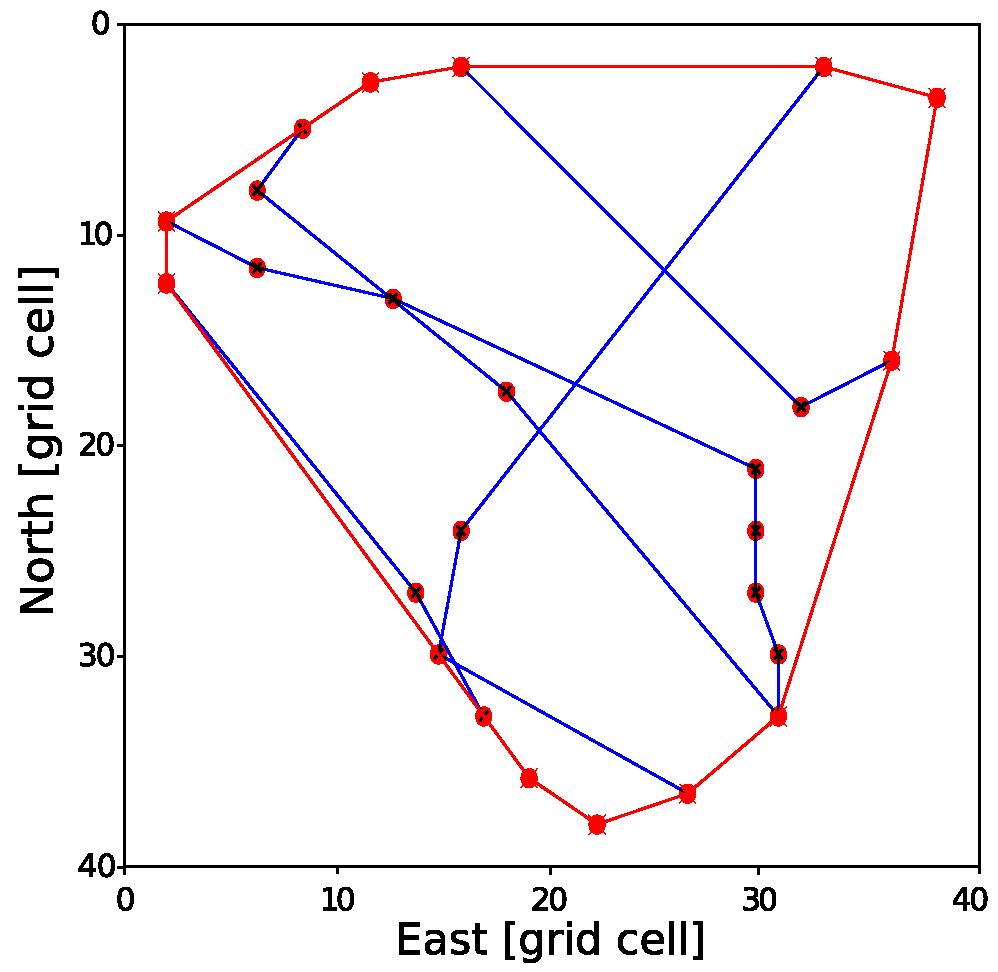
\includegraphics[width = %0.36\textwidth]{Figures/chull.%pdf}\label{fig:chull_path}}
%  \caption{Results from path %planning combining traveling %salesman and complex hull.}
%  \label{fig:path}
%\end{figure}

% The main components the sampling strategy is encapsulated in the pseudo-code in Algorithm \ref{alg:1}.

%\begin{algorithm}[!h]
%\small
%\SetAlgoLined
%\SetCommentSty{textit}
%\SetKwComment{Comment}{\%}{}
%\DontPrintSemicolon
%Initialize GP: Temperature, %Salinity\;
%% \emph{update\_GP\_bias()} %\Comment*[r]{Runs only once}
%\While{active}{
%\eIf{\textit{update} %\textbf{is} \textit{True}}{
%    \textit{points} = \emph{find\_points}($GP_{a,b}$, $t$, $s$) \Comment*[r]{Find the points where $\mid p(x) - 0.5 \mid$ is small}
%    \textit{path} = \emph{traveling\_balesman}(\emph{points})\;
%    \textit{path} = \emph{check\_path}(\emph{path}) \Comment*[r]{Check if the path is suitable for AUV (may need to use complex hull).}
%    }{\texttt{AUV\_Follow} \textit{path}.\;
      %\texttt{Assimilate\_GP} \textit{measurements}\;
%    \textit{update} = \emph{tigger\_update}() \Comment*[r]{\texttt{True} or \texttt{False} based on a criteria (time, destination, etc.)}}
%    }
%\caption{Excursion Probability Based Sampling Algorithm.}
%\label{alg:1}
%\end{algorithm}